\newpage
\thispagestyle{sectioned}
\chapter{Creación de aplicación Android (AppName)}

\section{Introducción}
Una vez que habíamos elegido la tecnología que soportaría el núcleo de nuestra aplicación, teníamos que decir que implementación le íbamos a dar a nuestra aplicación móvil. Para ello teníamos que tener en cuenta las características que nos ofrecía Wave:

Edición colaborativa.

Tiempo real.

Consistencia.

Después de darle unas cuantas vueltas de las posibles implementaciones que podríamos realizar sobre estas características potenciales, decidimos realizar una sesión de brain storming. En esta sesión aparecieron temas tan dispersos como wikis colaborativas, aplicaciones con inteligencia artificial, aportaciones colaborativas en política, edición de vídeos y música, cursos de formación colaborativos, etcétera.

	\begin{figure}[H]
      \centering
	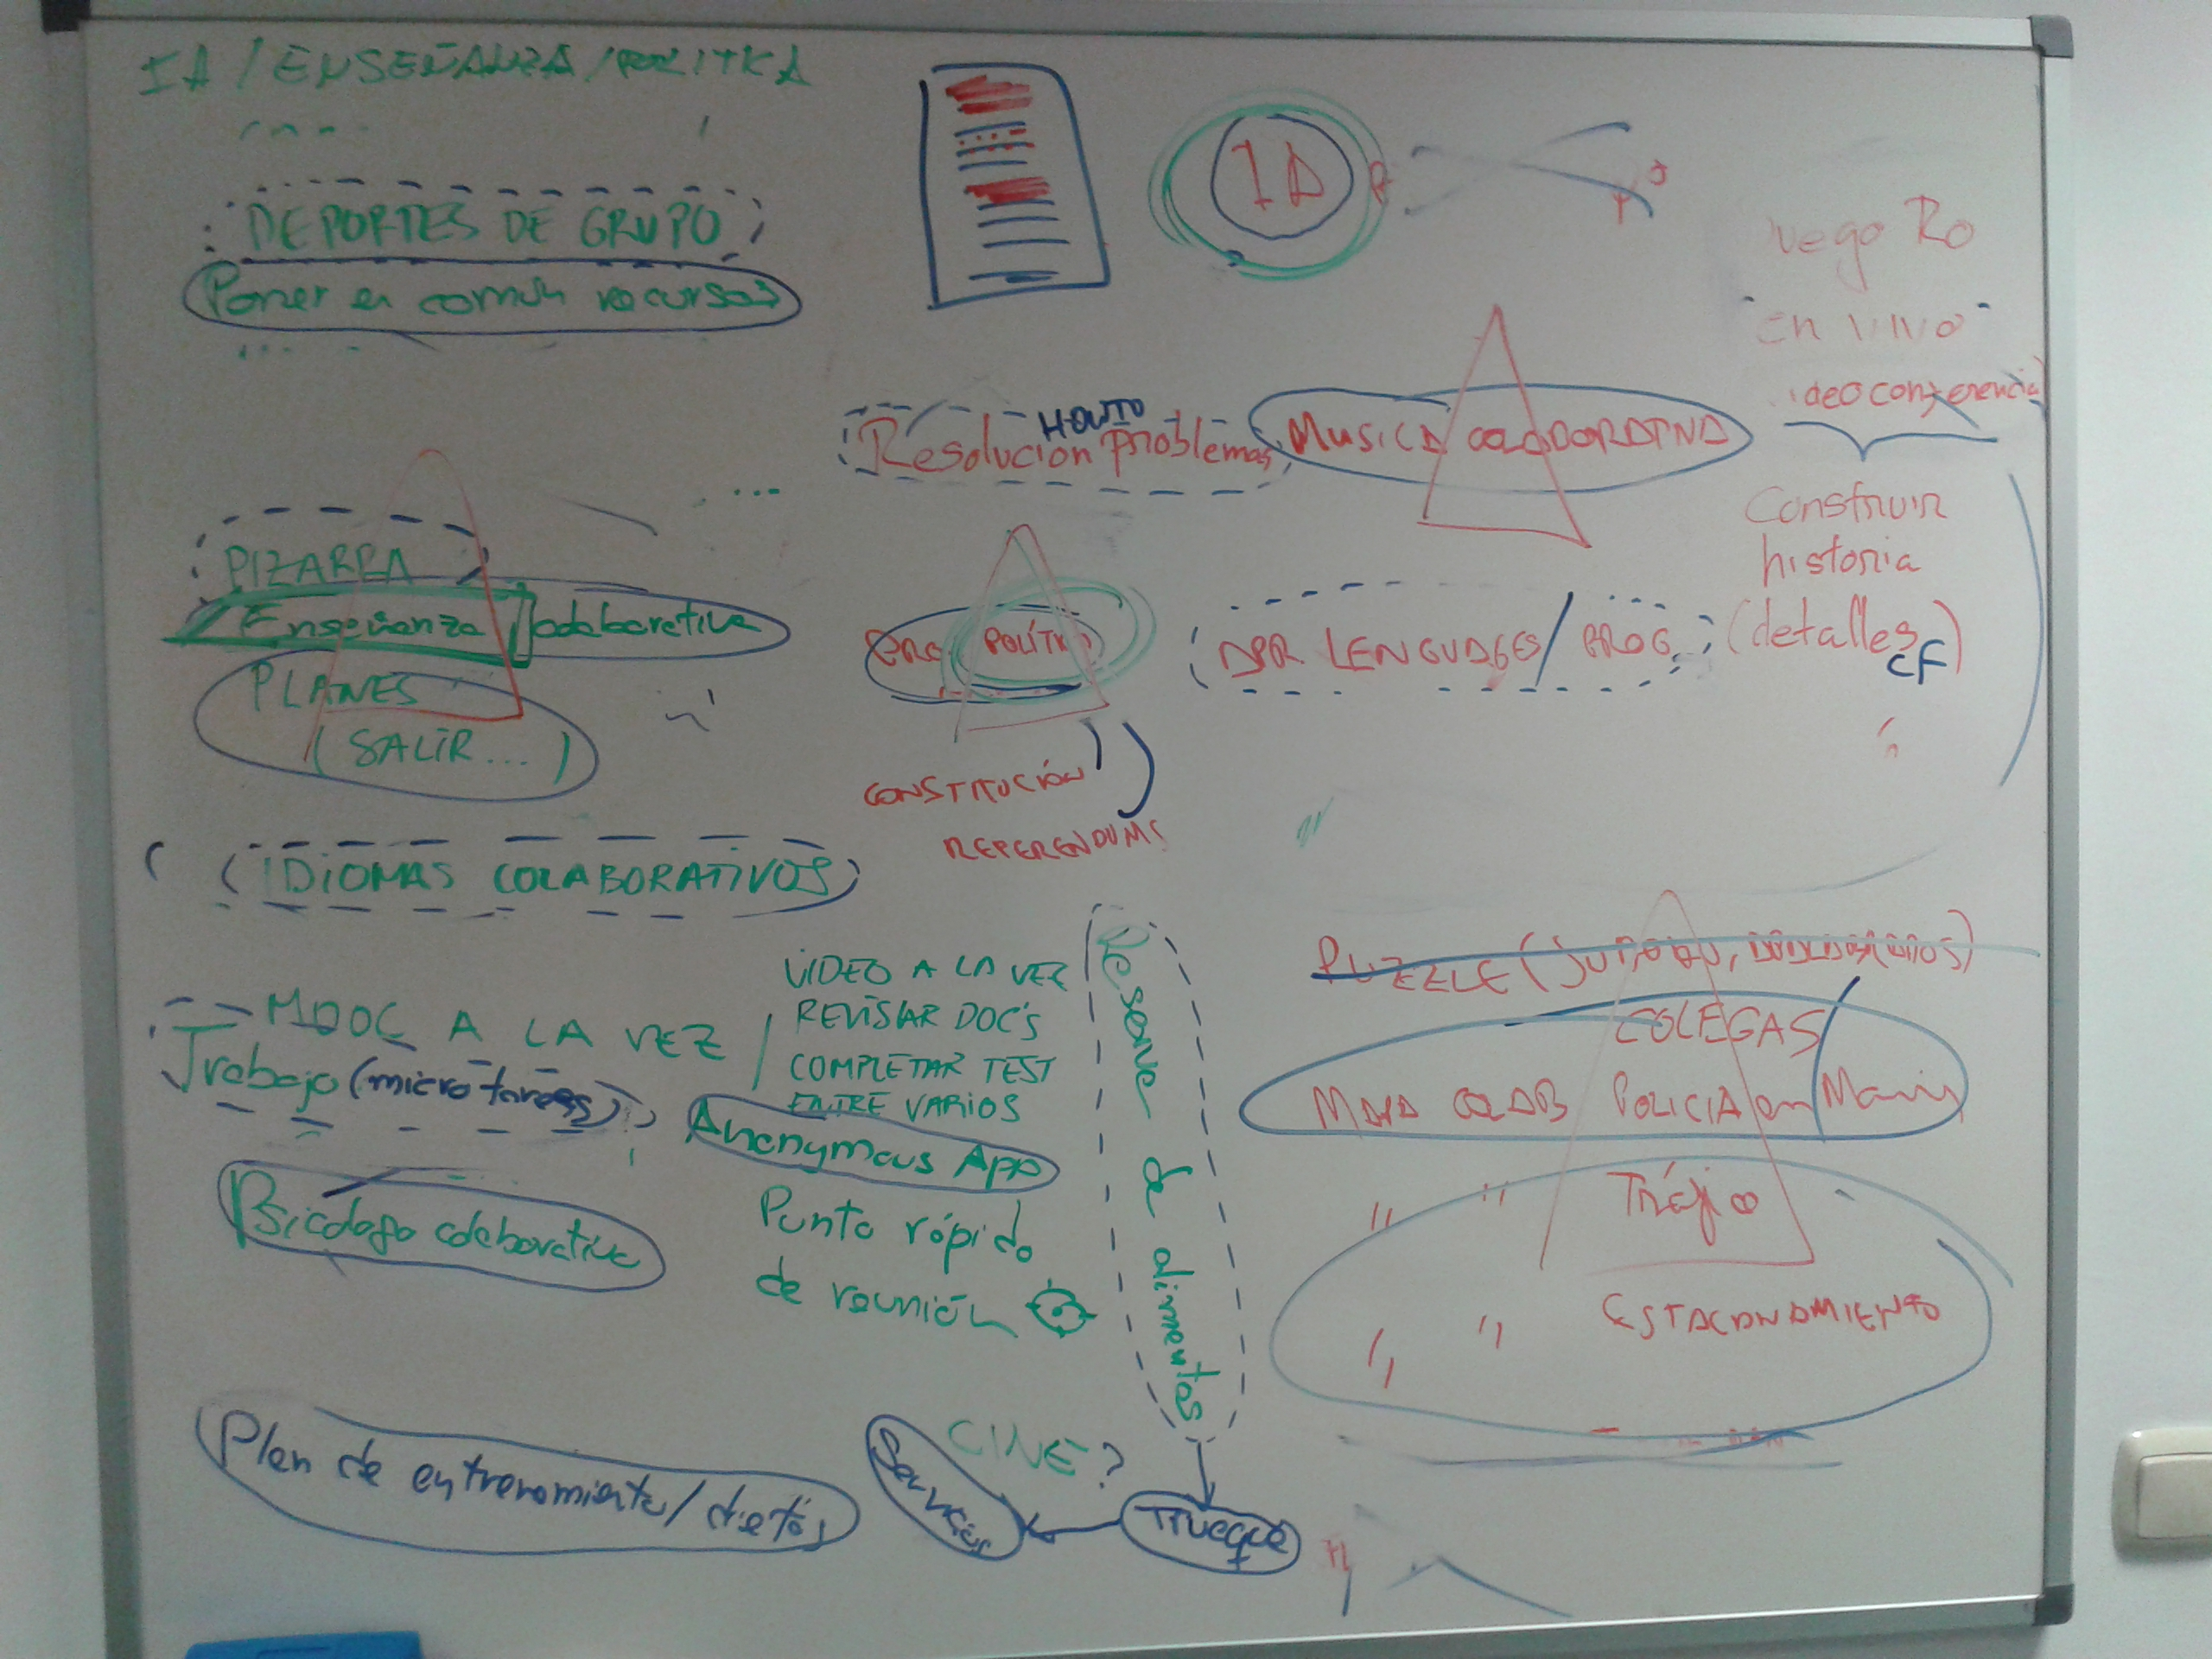
\includegraphics[keepaspectratio, scale=0.15]{Media/Captures/brainstorming.jpg}
      \caption{Brainstorming sobre la idea a desarrollar}
      \label{fig:brainstorming}
    \end{figure}
    
Con un gran repertorio de ideas expuestas sobre la sesión, descartamos aquellas que no nos motivaban llevarlas a cabo. Por lo que nos quedamos con tres ideas fundamentales a desarrollar en nuestra aplicación: Política, Música, Inteligencia Artificial y Mapas. Surgieron varias ideas colaborativas como desarrollar documentos políticos, programas electorales, comunicación entre colectivos en tiempo real, aprendizaje de música, edición de partituras y obras, aplicaciones colaborativas con inteligencia artificial, edición de mapas en tiempo real, lexicalización, etcétera.

Finalmente debido a intereses comunes, decimos realizar una aplicación colaborativa relacionado con el mundo de la política. Con el objetivo de que pudiera tener cierta repercusión y utilidad en las próximas citas electorales durante el año 2015. En esta aplicación podríamos recurrir a la edición de contenidos en tiempo real, ya fueran propuestas políticas, programas electorales y otro tipo de documentos. Como también hacer uso de alguna herramienta de Inteligencia Artificial para automatizar algunas tareas o realizar recomendaciones sociales.

\subsection{Adentrándonos en la idea}
La idea a desarrollar generada en una época dónde la política parecía haber despertado el interés de una parte considerable de la ciudadanía, podría ser una herramienta útil para participar en temas políticos que forma sencilla y atractiva. Dejando atrás los tópicos yo no entiendo de política, la política es aburrida, no sé a quién votar o no he leído nunca un programa electoral entre otros.

La herramienta ofrecería una nueva forma de participar en la política y de llevar a los ciudadanos los programas electorales ofertados por las diferentes formaciones políticas. De tal forma que los ciudadanos pudieran leer aquellos puntos de los programas más leídos, debatidos, comentados, etcétera. Así cualquier usuario tendría todos programas electorales en su bolsillo, por lo que no tendría que ir a la página web de cada formación política y descargarse un documento de 200 páginas. Pensamos que esta forma de presentar un programa político en un mundo donde las posibilidades de  comunicarnos se han desarrollado exponencialmente, no era la mejor manera de llegar a la mayor parte de la ciudadanía.

Por otra parte, la aplicación también debería ofrecer alguna herramienta donde realizar propuestas y debatirlas entre todos. De tal forma que tanto la ciudadanía como las formaciones políticas pudieran saber en cualquier momento cuáles son las principales preocupaciones de los ciudadanos y qué medidas o soluciones proponen para resolverlas.

Desde un primer punto de vista subjetivo, la aplicación quedó dividida en dos partes. Por un lado tendríamos los programas políticos que presentaran las formaciones políticas. Y por otro, todas las propuestas que elaboraran los ciudadanos individualmente o en colectivos sociales.

\section{1ª Parte: Programas Políticos}
En esta sección se desarrollará en profundidad todo lo relacionado con los partidos políticos.

  \subsection{Estado del Arte}
En la actualidad no existe ningún tipo de aplicación orientada a debatir los programas electorales de los partidos políticos. Concretamente no hay ningún tipo de plataforma que agrupe los programas electorales de las diferentes candidaturas.
Lo más parecido que hemos podido encontrar han sido aplicaciones elaboradas por un partido político, orientada a dar a conocer su candidatura. En ella podremos ver la candidatura, vídeos y el programa electoral entre otros. Por ello pasamos a analizar las aplicaciones encontradas:

	\subsubsection{UPyD Parla}\label{sssec:UPyDParla}
La aplicación que presenta el candidato de UpyD Carlos Alt Bustelo para la alcaldía de Parla. Se trata de una alicación divulgativa donde podemos conocer todo lo esencial de la candidatura de UpyD para las elecciones del municiono de Parla en Mayo de 2015. Los candidatos, el programa, vídeos, etcétera.

	\begin{figure}[H]
      \centering
	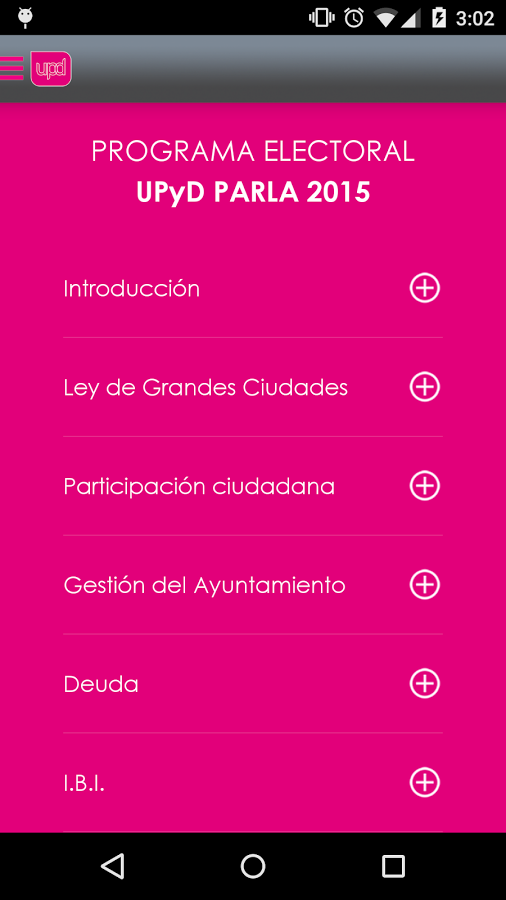
\includegraphics[keepaspectratio, scale=0.35]{Media/Captures/UPyDParla.png}
      \caption{UPyD Parla}
      \label{fig:upydparla}
    \end{figure}

	\subsubsection{$\sharp$RecuperaCórdoba}\label{sssec:RecuperaCordoba}
De forma similar a la anterior, la candidatura de Pedro García a la provincia de Córdoba de Izquierda Unida, presenta su propuesta de gobierno de forma compacta. En la aplicación podremos encontrar la lista de los candidatos propuestos a la comunidad cordobesa, el programa electoral de la formación, las propuestas del partido, noticias de última hora y vídeos.

	\begin{figure}[H]
      \centering
	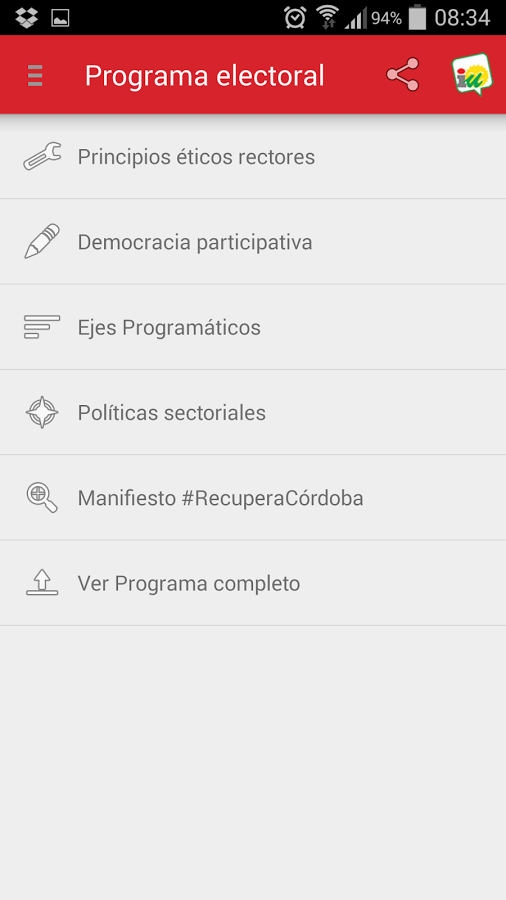
\includegraphics[keepaspectratio, scale=0.35]{Media/Captures/IURecuperaCordoba.png}
      \caption{$\sharp$RecuperaCórdoba}
      \label{fig:recuperacordoba}
    \end{figure}
    
    	\subsubsection{PP Canarias}\label{sssec:pp_canarias}
    	
La delegación del Partido Popular en Canarias, presenta su aplicación móvil para promocionar a sus candidatos para las elecciones autonómicas y municipales de Mayo de 2015. La aplicación nos avisará de los eventos electorales, podremos consultar los candidatos, novedades, galería de imágenes y por su puesto el programa electoral.

	\begin{figure}[H]
      \centering
	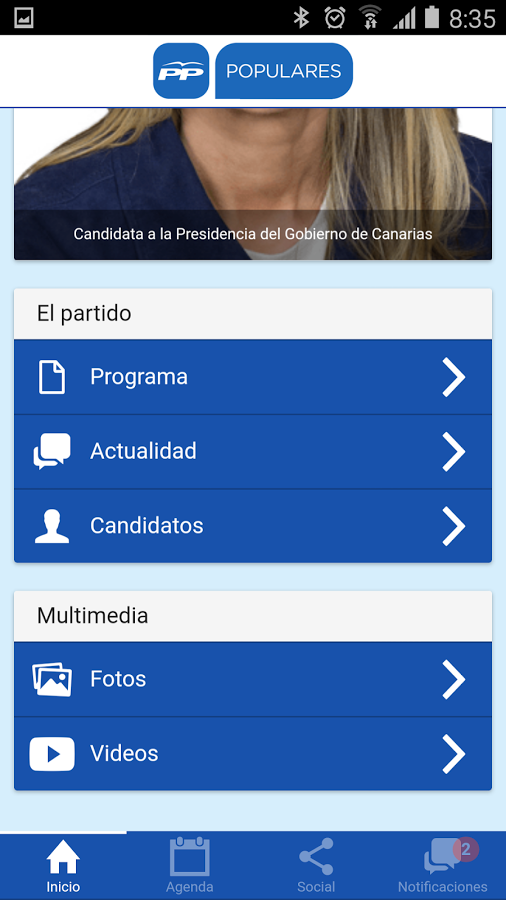
\includegraphics[keepaspectratio, scale=0.35]{Media/Captures/ppcanarias.png}
      \caption{PP Canarias}
      \label{fig:ppcanarias}
    \end{figure}

	\subsection{Intención}

La intención fundamental de la aplicación es llevar los programas electorales a los bolsillos de los ciudadanos. Vivimos en una sociedad digital, donde cada vez son más las personas que utilizan los teléfonos inteligentes para realizar todo tipo de tareas en su vida cotidiana.

En los últimos años las diferentes formaciones políticas han subido sus programas electorales a un documento en formato pdf que estaba disponible en su página web. Este documento generalmente extenso, no es un medio fácil de divulgar y mostrar a la ciudadanía. Por ello pensamos que una aplicación que pudiera visualizar las principales secciones de los programas políticos, podría ser especialmente útil para acercar los programas a los electores.

Llegando a crear un espacio donde poder informase sobre las distintas ofertas electorales, debatir las propuestas que propone cada formación política reducido en una aplicación que podremos consultar en cualquier momento.
  
	\subsection{Objetivos}
	
La aplicación pretende llevar las principales partes de los programas electorales de los partidos que se presenten a las elecciones. Por tanto, cualquier usuario podrá visualizar el apartado que desee consultar de cualquier partido político. Siendo esta la forma menos amigable de leerlo, se utilizarán distintas formas para compartir o divulgar determinadas secciones más populares.

Al inicio de la aplcación, mostrará una lista de las secciones de los programas más valoradas, más debatidas, peor valoradas e incluso las más incomprendidas. Por tanto creemos que puede ser una forma de acercar aquellas secciones más populares de forma más eficaz, al contrario que tener que consultar una determinada página dentro de un extenso pdf.

	\begin{figure}[H]
      \centering
	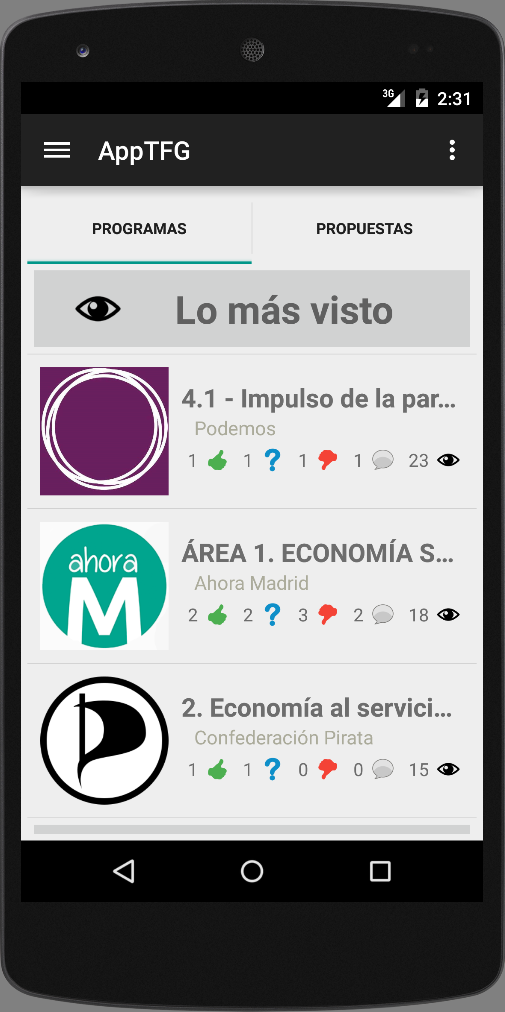
\includegraphics[keepaspectratio, scale=0.5]{Media/Captures/captTopSections.png}
      \caption{Vista principal de secciones}
      \label{fig:captTopSections}
    \end{figure}
    
Dentro de cada sección podemos visualizar el contenido de la sección a la que referencia el programa, y tendremos la opción de valorarla de forma positiva o negativa. También añadimos la posibilidad de indicar que no se ha entendido la sección. Pues a la hora de leer una propuesta de gobierno ubicada en una sección del programa, bien nos puede gustar, disgustar o simplemente no haber entendido la idea y por ello no votarla de forma positiva o negativa.

	\begin{figure}[H]
      \centering
	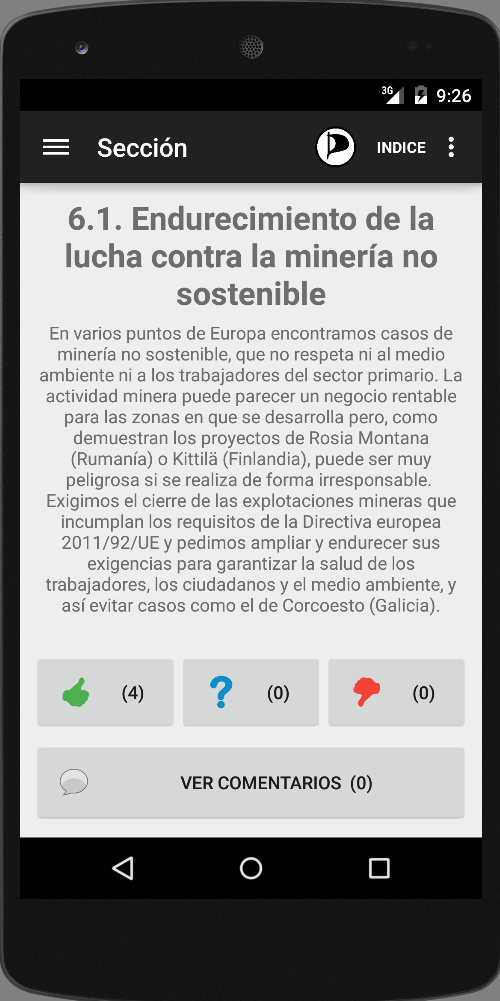
\includegraphics[keepaspectratio, scale=0.5]{Media/Captures/section.png}
      \caption{Visualizando una sección}
      \label{fig:captSection}
    \end{figure}
    
Sin olvidarnos de la parte social, en cada sección podemos hacer comentarios para intentar debatir las ideas fundamentales que propone la sección. O incluso hacer referencia a una determinada frase o párrafo.
	\subsection{Usabilidad}
	
	\subsection{Revisión de la aplicación}
Una vez que habíamos implementado todos los objetivos fundamentales de la aplicación, decidimos hacer una revisión para poner a prueba la aplicación. Para ello nos reunimos con un grupo de \cite{ref:labodemo}, responsables del desarrollo de los portales de participación ciudadana del partido político \cite{ref:podemos} y la candidatura de unidad popular \cite{ref:ahoramadrid}.



  
\section{2ª Parte: Propuestas y Comparativas}
  \subsection{Estado del Arte}

  \subsection{Intencion}
  \subsection{Objetivos}
  \subsection{Usabilidad}

  
  
\section{Tecnologias y Metodologías de la app}

  \subsection{Base de Datos}
  \subsection{Service REST}

  \subsection{Frontend}
